\PassOptionsToPackage{lowtilde}{url}
\documentclass[aspectratio=43,english]{beamer} %If you want to create Polish presentation, replace 'english' with 'polish' and uncomment 3-th line, i.e., '\usepackage{polski}'
\usepackage[utf8]{inputenc}
\usepackage{polski} %Uncomment for Polish language
\usepackage{babel}
\usepackage{listings} %We want to put listings

\mode<beamer>{ 	%in 'beamer' mode
	\hypersetup{pdfpagemode=FullScreen}		%Enable Full screen mode
	\usetheme{JuanLesPins} 		%Show part title in right footer
	%\usetheme[dark]{AGH}                 		%Use dark background
	%\usetheme[dark,parttitle=leftfooter]{AGH}  	%Use dark background and show part title in left footer
}
\mode<handout>{	%in 'handout' mode
	\hypersetup{pdfpagemode=None}
	\usepackage{pgfpages}
  	\pgfpagesuselayout{4 on 1}[a4paper,border shrink=5mm,landscape]	%show 4 slides on 1 page
  	\usetheme{boxes}
  	\addheadbox{structure}{\quad\insertpart\hfill\insertsection\hfill\insertsubsection\qquad} 	%content of header
 	\addfootbox{structure}{\quad\insertauthor\hfill\insertframenumber\hfill\insertsubtitle\qquad} 	%content of footer
}

\AtBeginPart{ %At begin part: display its name
	\frame{\partpage}
}


%%%%%%%%%%% Configuration of the listings package %%%%%%%%%%%%%%%%%%%%%%%%%%
% Source: https://en.wikibooks.org/wiki/LaTeX/Source_Code_Listings#Using_the_listings_package
%%%%%%%%%%%%%%%%%%%%%%%%%%%%%%%%%%%%%%%%%%%%%%%%%%%%%%%%%%%%%%%%%%%%%%%%%%%%
\lstset{ %
  backgroundcolor=\color{white},   % choose the background color
  basicstyle=\footnotesize,        % the size of the fonts that are used for the code
  breakatwhitespace=false,         % sets if automatic breaks should only happen at whitespace
  breaklines=true,                 % sets automatic line breaking
  captionpos=b,                    % sets the caption-position to bottom
  commentstyle=\color{green},      % comment style
  deletekeywords={...},            % if you want to delete keywords from the given language
  escapeinside={\%*}{*)},          % if you want to add LaTeX within your code
  extendedchars=true,              % lets you use non-ASCII characters; for 8-bits encodings only, does not work with UTF-8
  frame=single,	                   % adds a frame around the code
  keepspaces=true,                 % keeps spaces in text, useful for keeping indentation of code (possibly needs columns=flexible)
  keywordstyle=\color{blue},       % keyword style
  morekeywords={*,...},            % if you want to add more keywords to the set
  numbers=left,                    % where to put the line-numbers; possible values are (none, left, right)
  numbersep=5pt,                   % how far the line-numbers are from the code
  numberstyle=\tiny\color{gray},   % the style that is used for the line-numbers
  rulecolor=\color{black},         % if not set, the frame-color may be changed on line-breaks within not-black text (e.g. comments (green here))
  showspaces=false,                % show spaces everywhere adding particular underscores; it overrides 'showstringspaces'
  showstringspaces=false,          % underline spaces within strings only
  showtabs=false,                  % show tabs within strings adding particular underscores
  stepnumber=2,                    % the step between two line-numbers. If it's 1, each line will be numbered
  stringstyle=\color{cyan},        % string literal style
  tabsize=2,	                   % sets default tabsize to 2 spaces
  title=\lstname,                  % show the filename of files included with \lstinputlisting; also try caption instead of title
                                   % needed if you want to use UTF-8 Polish chars
  literate={?}{{\k{a}}}1
           {?}{{\k{A}}}1
           {?}{{\k{e}}}1
           {?}{{\k{E}}}1
           {�}{{\'o}}1
           {�}{{\'O}}1
           {?}{{\'s}}1
           {?}{{\'S}}1
           {?}{{\l{}}}1
           {?}{{\L{}}}1
           {?}{{\.z}}1
           {?}{{\.Z}}1
           {?}{{\'z}}1
           {?}{{\'Z}}1
           {?}{{\'c}}1
           {?}{{\'C}}1
           {?}{{\'n}}1
           {?}{{\'N}}1
}
%%%%%%%%%%%%%%%%%
\setcounter{tocdepth}{1}

\newcommand\tab[1][0.5cm]{\hspace*{#1}}


\newcommand{\setcontributors}[1]{
	\let\oldmaketitle\maketitle
	\renewcommand{\maketitle}{
		\begin{frame}
			\oldmaketitle

			\noindent
				\begin{minipage}{0.4\textwidth}
						\footnotesize{\textbf{Contributors}}\\
						\scriptsize{#1}
						% \footnotesize{\textbf{Source code}}\\
						% 	\tab \scriptsize{\href{https://github.com/AGH-MOwNiT-2017/lectures}{\texttt{github.com/AGH-MOwNiT-2017/lectures}}}

				\end{minipage}
				\hfill%
				\begin{minipage}{0.45\textwidth}\raggedleft% adapt widths of minipages to your needs
					\includegraphics[width=25px, height=25px]{img/title/dice}
					\includegraphics[width=60px, height=35px]{img/title/ki}
					\includegraphics[width=30px, height=30px]{img/title/agh}

				\end{minipage}%


		\end{frame}
	}
}


\title{Metody Obliczeniowe w Nauce i Technice}
\author{Marian Bubak, Katarzyna Rycerz}
\date{}
\institute[AGH]{
	Department of Computer Science\\
	AGH University of Science and Technology\\
	Krakow, Poland\\
	\href{mailto:kzajac@agh.edu.pl}{\texttt{kzajac@agh.edu.pl}}\\
	% \href{http://www.icsr.agh.edu.pl/~mownit/}{\texttt{icsr.agh.edu.pl/$\sim$mownit}}
	\href{http://dice.cyfronet.pl/}{\texttt{dice.cyfronet.pl}}

}
\usepackage{tikz}
\usetikzlibrary{shapes.arrows}
\tikzset{
    myarrow/.style={
        draw,
        fill=black,
        single arrow,
        minimum height=4.5ex,
        single arrow head extend=1ex
    },
     myarrow2/.style={
        draw,
        fill=black,
        double arrow,
        minimum height=8.5ex,
        double arrow head extend=1ex
    }
}
\usepackage[braket]{qcircuit}
\newcommand{\arrowup}{%
\tikz [baseline=-0.5ex]{\node [myarrow,rotate=90] {};}
}
\newcommand{\arrowdown}{%
\tikz [baseline=-1ex]{\node [myarrow,rotate=-90] {};}
}
\newcommand{\arrowupdown}{%
\tikz [baseline=-1ex]{\node [myarrow2,rotate=-90] {};}
}
\subtitle{Optymalizacja metodą simulated annealing}
\setcontributors{Marcin Przewięźlikowski\\Miłosz Błaszkiewicz\\Łukasz Janeczko}


\begin{document}
  	\maketitle
	%%%%%%%%%%%%%%%%
	\begin{frame}{Outline}
		\tableofcontents
	\end{frame}
	%%%%%%%%%%%%%%%%
	\input{18_simulated_annealing/18_1_wprowadzenie}
	%%%%%%%%%%%%%%%%%%%%%%%
	\section{Optymalizacja kombinatoryczna}

%%%%%%%%%%%%%%%%
%	\begin{frame}{Optymalizacja kombinatoryczna }
	%	\begin{exampleblock}{Przykład: Problem komiwojażera}
	%		\begin{itemize}
		%		\item \textbf{In}: %symetryczna macierz odległości $(N*N)$

		%		\item \textbf{Out}: permutacja zbioru $\{1,2,...,N\}$ taka, że np:
		%			$$
		%				L_{min} = \sum_{i=1}^N \{ \underbrace{(|x_i - x_{i+1}| + |y_i - y_{i+1}|)}_\text{odległość w metryce Manhattan} + \underbrace{\lambda(\mu_i - \mu_{i-1})}_\text{funkcja kary (penalty)}\}
		%			$$
		%	\end{itemize}
			%DEAD LINK
			%Demo optymalizacji problemu %komiwojażera (autor: Maciej %Borowiec): %\url{komiwojazer/komiwojazer.html}
	%	\end{exampleblock}

	%\end{frame}
%%%%%%%%%%%%%%%%

	\begin{frame}{Optymalizacja kombinatoryczna}
		%\begin{exampleblock}{Zagadnienia NP-zupełne (nondeterministic polynomial)}
			\begin{itemize}
				\item rozwiązania o złożoności $\sim e^N$
				\item wiele stopni swobody
				\item dyskretne (wykluczone poszukiwanie w kierunku)
				\item funkcja celu  łączy przeciwstawne cele cząstkowe
			\end{itemize}
	%	\end{exampleblock}
	%	Dobry przegląd w \cite{garey}
	%	\begin{thebibliography}{9}
			%\setbeamertemplate{bibliography item}[article]
		%	\bibitem{garey}{M.R. Garey, D.S. Johnson \newblock Computers and Intractability: A Guide to the Theory of NP \newblock Completeness, Freeman, San Francisco, 1979}
	%	\end{thebibliography}
	\end{frame}

%%%%%%%%%%%%%%%%
	\begin{frame}{Przykład: problem Max-Cut}
 \begin{figure}
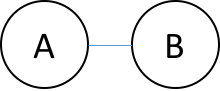
\includegraphics[scale=0.3]{img/18/barbell.png}
%\caption{Graph to cut}
\end{figure} 
\begin{figure}
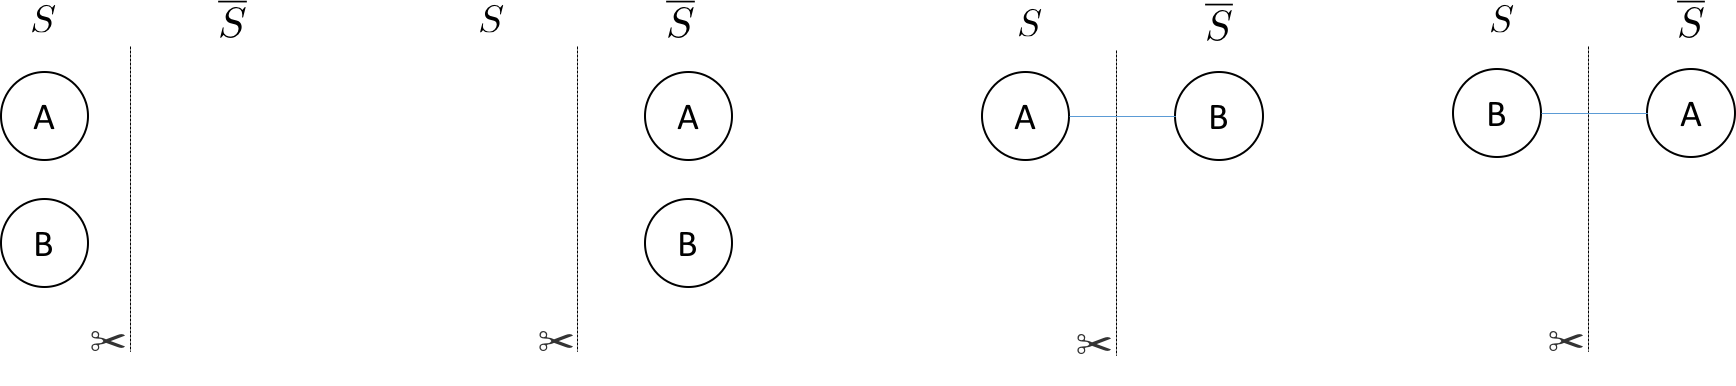
\includegraphics[scale=0.18]{img/18/partition_barbell.png}
%\caption{Cutting possibilities}
\end{figure} 
Funkcja kosztu:
    \begin{itemize}
        \item[] $g(x_1, x_2)=x_1+x_2-2x_1 x_2$, $x_1,x_2 \in\{0,1\}$
        \item[] $g(00)=0$ $g(11)=0$
        \item[] $g(01)=1$ $g(10)=1$
    \end{itemize}
    \\
    \small{source: https://grove-docs.readthedocs.io/en/latest/qaoa.html}
\end{frame}
\begin{frame}{Przykład - problemy BILP i QUBO}
\begin{block}{Funkcja kosztu i warunki (zmienne binarne)}
$f(x)=c^Tx$ and  $Ax=b$ $x_i \in \{0,1\}$
\end{block}
\begin{center}
    \arrowdown $C$-diagonal, diag($C$)=$c$
\end{center}
\begin{block}{QUBO - quadratic and uncontraint cost function $f(x)=x^TQx$}
$f(x)=x^TCx+P\underbrace{(Ax-b)^T(Ax-b)}_{\substack{\text{instead of solving } Ax=b \\ \text{we minimize inner product of }
Ax-b
}}$ 
\end{block}
\end{frame}

\subsection{Typowa funkcja celu}
	\begin{frame}{Typowa funkcja celu}
		\begin{itemize}
			\item skalar: wszystkie cele sprowadza do jednego
			\item wiele lokalnych minimów - rzędu $e^N$
			\item w praktyce - potrzebne dobre rozwiązanie - nie musi być to minimum globalne
		\end{itemize}

	\end{frame}

%%%%%%%%%%%%%%%%

	\begin{frame}{Typowa funkcja celu}
		\begin{figure}
			\includegraphics[height=0.9\textheight]{img/18/target_fun}
		\end{figure}
	\end{frame}

%%%%%%%%%%%%%%%%

	

%%%%%%%%%%%%%%%%

	\begin{frame}{Przykład procedury generacji nowych konfiguracji}
		\begin{exampleblock}{TSP \cite{lin}}
			Heurystyka: \textit{iterative improvement} - akceptowalne zmiany zmniejszające funkcję celu
			\begin{enumerate}
				\item odwrócenie kolejności obiegu 5-ciu górnych
				\item wstawienie 5-ciu górnych między 2 dolne
			\end{enumerate}
			$\rightarrow$ pewne ugrzęźnięcie w lokalnym minimum
			\begin{figure}
				\includegraphics[height=0.32\textheight]{img/18/tsp}
			\end{figure}
		\end{exampleblock}
		\begin{thebibliography}{9}
			\setbeamertemplate{bibliography item}[book]
			\bibitem{lin}{S. Lin, B.W. Kernighan, Oper. Res. 21 (1973) 498}
		\end{thebibliography}
	\end{frame}

	%%%%%%%%%%%%%%%%%%%%%%%
	\section{Annealing \& quenching}

%%%%%%%%%%%%%%%% 

	\begin{frame}{Annealing \& quenching}
		\textbf{Czyli powolne i szybkie schładzanie}
		\begin{block}{Annealing}
			Stopniowe, powolne zmniejszanie temperatury
			\begin{itemize}
				\item topnienie (ciecz)
				\item w każdej temperaturze trwa długo, do uzyskania równowagi termicznej
			\end{itemize}
			$\Rightarrow$ uporządkowanie w kryształ - struktura regularna, symetryczna o minimalnej energii
		\end{block}
	\end{frame}

%%%%%%%%%%%%%%%% 

	\begin{frame}{Annealing \& quenching}
		\begin{block}{Quenching}
			Szybkie zmniejszanie temperatury \\
			$\Rightarrow$ uzyskanie stanu metastabilnego
			\begin{itemize}
				\item polikryształ
				\item kryształ z defektami
			\end{itemize}
			Odpowiednik \textit{iterative improvement}
		\end{block}
		\textbf{Wniosek:} zamiast zawsze odrzucać konfigurację zwiększającą funkcję celu, niekiedy należy ją akceptować z odpowiednim prawdopodobieństwem (uphill)
	\end{frame}
	%%%%%%%%%%%%%%%%%%%%%%%
	\section{Fizyka statystyczna i optymalizacja - analogie}

%%%%%%%%%%%%%%%% 
	\begin{frame}{Fizyka statystyczna i optymalizacja - analogie}
		\begin{block}{Fizyka statystyczna}
				uśrednione wartości dla zespołów o dużej ilości molekuł	
		\end{block}
		
		
		\begin{table}[]
		\centering
		\begin{tabular}{|l|l|}
		\hline
		\textbf{Mechanika statystyczna}                                                                                                 & \textbf{Optymalizacja}                                                                  \\ \hline
		wiele oddziałujących molekuł                                                                                                    & wiele parametrów                                                                        \\ \hline
		układ, zbiór położeń molekuł                                                                                                    & konfiguracja                                                                            \\ \hline
		\begin{tabular}[c]{@{}l@{}}schłodzenie do stabilnego stanu \\ niskoenergetycznego\end{tabular}                                  & \begin{tabular}[c]{@{}l@{}}znalezienie konfiguracji \\ prawie optymalnej\end{tabular}   \\ \hline
		temperatura                                                                                                                     & \begin{tabular}[c]{@{}l@{}}parametr sterujący \\ przebiegiem optymalizacji\end{tabular} \\ \hline
		hamiltonian (operator energii) \\                                                                             & funkcja celu                                                                            \\ \hline
		\begin{tabular}[c]{@{}l@{}}w hamiltonianie człony \\
		wynikające z róznych oddziaływań
		\end{tabular} & \begin{tabular}[c]{@{}l@{}}współzawodniczące człony \\ w funkcji celu\end{tabular}      \\ \hline
		\end{tabular}
		\end{table}

	\end{frame}
	\begin{frame}{Przykład: problem Max-Cut}
 \begin{figure}
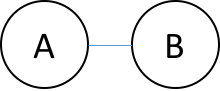
\includegraphics[scale=0.3]{img/18/barbell.png}
%\caption{Graph to cut}
\end{figure} 
\begin{figure}
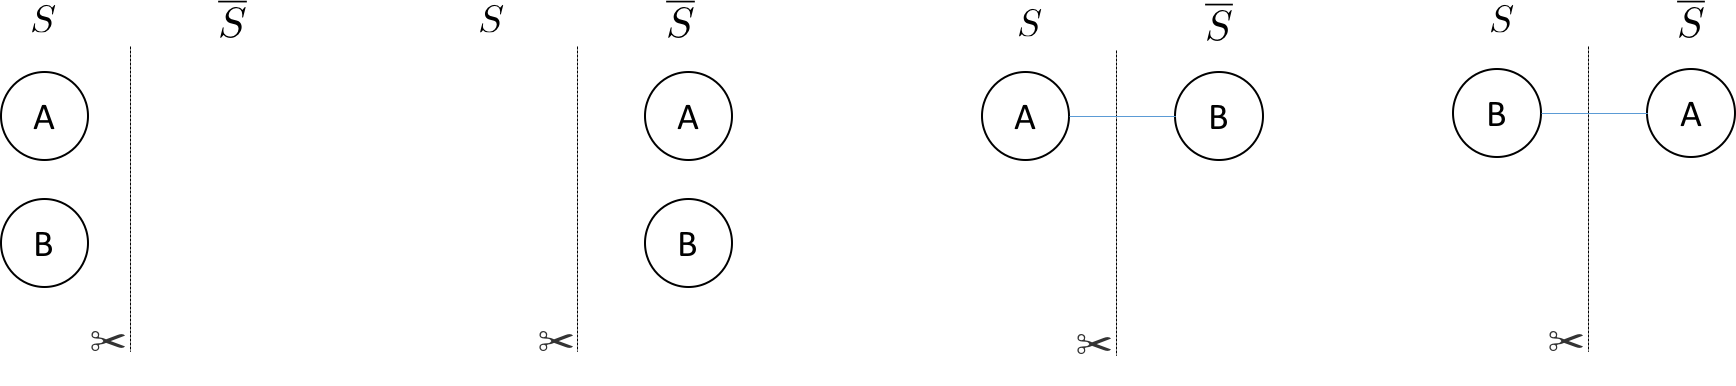
\includegraphics[scale=0.18]{img/18/partition_barbell.png}
%\caption{Cutting possibilities}
\end{figure} 
Funkcja kosztu:
    \begin{itemize}
        \item[] $g(x_1, x_2)=x_1+x_2-2x_1 x_2$, $x_1,x_2 \in\{0,1\}$
        \item[] $g(00)=0$ $g(11)=0$
        \item[] $g(01)=1$ $g(10)=1$
    \end{itemize}
    \\
    \small{source: https://grove-docs.readthedocs.io/en/latest/qaoa.html}
\end{frame}

\begin{frame}{Hamiltonian dla MaxCut}
Mamy efektywną symulację dla modelu Isinga:
\url{http://www.bdhammel.com/ising-model/}
  \url{https://stanford.edu/~jeffjar/statmech/intro4.html} \\
  Funkcja kosztu naszego problemu:
    \begin{itemize}
        \item[] $g(x_1, x_2)=x_1+x_2-2x_1 x_2$, $x_1,x_2 \in\{0,1\}$
       \end{itemize}
W modelu Isinga
       \begin{itemize}
           \item  x=0 - spin do góry (z=1)
           \item  x=1 - spin w dół (z=-1)
       \end{itemize}
    
Funkcja energii zależna od konfiguracji\_spinów     
       \begin{itemize}
        \item[] $x\rightarrow \frac{1}{2}(1-z)$  
        \item[] $g(z_1,z_2)=\frac{1}{2}(1-z_1z_2)$ $z_1,z_2 \in\{-1,1\}$
   \end{itemize}     
\end{frame}
\begin{frame}{Model Isinga}
$$ H_{\text{maxcut}}=\frac{1}{2}  - \frac{1}{2} \sum_{<ij>} {z_{i}} {z_{j}}$$

$$ H_{\text{Ising}}=- \sum_{i} h_i z_i - \sum_{<ij>} J_{i,j} z_{i} z_{j}
$$
$$H_{\text{maxcut}}=\frac{1}{2} - \frac{1}{2} H_{\text{Ising}}$$
dla $h=0$, $J=-1$\\

\end{frame}%\begin{frame}{Notacja Diraca, iloczyn tensorowy}
 %  $$\ket{0}=\begin{bmatrix}1\\0
  %      \end{bmatrix}
   %     \ket{1}=\begin{bmatrix}0\\1
    %    \end{bmatrix}$$ 
%        $$\ket{00}=\begin{bmatrix}1\\0\\0\\0
%        \end{bmatrix}
%        \ket{01}=\begin{bmatrix}0\\1\\0\\0
%        \end{bmatrix}
%        \ket{10}=\begin{bmatrix}0\\0\\1\\0
%        \end{bmatrix}
%        \ket{11}=\begin{bmatrix}0\\0\\0\\1
%        \end{bmatrix}$$ 
%        $$\ket{01}=\ket{0}\otimes\ket{1}=
%        \begin{bmatrix}1\\0
%        \end{bmatrix}\otimes
%\begin{bmatrix}0\\1
%        \end{bmatrix}=
%        \begin{bmatrix}1\cdot0\\1\cdot1\\0\cdot0%\\0\cdot1
%        \end{bmatrix}=\begin{bmatrix}0\\1\\0\\0
%        \end{bmatrix}$$
%        
%\end{frame}
%\begin{frame}{Hamiltonian dla MaxCut}
%Funkcja kosztu:
 %   \begin{itemize}
 %       \item[] $g(x_1, x_2)=x_1+x_2-2x_1 x_2$, $x_1,x_2 \in\{0,1\}$
  %      \item[] $x\rightarrow \frac{1}{2}(1-z)$  
   %     \item[] $g(z_1,z_2)=\frac{1}{2}(1-z_1z_2)$ $z_1,z_2 \in\{-1,1\}$
    %    \item[]
     %   $\sigma_z=\begin{pmatrix}  
%    1 &0\\
 %    0 & -1\\
  %  \end{pmatrix}$
   %     \item[] $\sigma_z\ket{0}=\ket{0}, \lambda=1$
    %    \item[] $\sigma_z\ket{1}=-\ket{1}, %\lambda=-1$
     %   \item[] aby zbudować Hamiltonian: $z\rightarrow \sigma_z$
      %  \item[] $H_{i,j}=\frac{1}{2}(I-{\sigma_z}^i\otimes {\sigma_z}^j)=\begin{pmatrix}  
    %0 &0&0&0\\
    % 0 &1&0&0\\
     % 0 &0&1&0\\
     %  0 &0&0&0
    %\end{pmatrix} \begin{matrix}
    %\ket{00}\\
    % \ket{01}\\
    %  \ket{10}\\
    %   \ket{11}\\
    %\end{matrix}$
     %   \item[]Wartości włąsne
      %  \begin{itemize}
       %     \item $0$ dla $\ket{00}$ i %$\ket{11}$ ; $g(00)=0$ $g(11)=0$
    %         \item $1$ dla $\ket{01}$ i %$\ket{10}$ ; $g(01)=1$ $g(10)=1$
    %    \end{itemize}
    %\end{itemize}
    %\\
    %\small{source: %https://grove-docs.readthedocs.io/en/latest/qaoa.html}
%\end{frame}
%%$$ H_{\text{maxcut}}=\frac{1}{2} I - \frac{1}{2} \sum_{<ij>} {\sigma_{z}_{(i)}} {\sigma_{z}_{(j)}}$$

%$$ H_{\text{Ising}}=- \sum_{i} h_i %{\sigma_{z}_{(i)}} - \sum_{<ij>} J_{i,j} %{\sigma_{z}_{(i)}} {\sigma_{z}_{(j)}}
%$$
%$$H_{\text{maxcut}}=\frac{1}{2} - \frac{1}{2} H_{\text{Ising}}$$
%dla $h=0$, $J=-1$\\
%\url{http://www.bdhammel.com/ising-model/}
%  \url{https://stanford.edu/~jeffjar/statmech/intro4.html} 
%\end{frame}

	%%%%%%%%%%%%%%%%%%%%%%%
	\section{Algorytm Simulated Annealing}

%%%%%%%%%%%%%%%%
\begin{frame}{Typowa funkcja celu}
		Niezbędne:
		\begin{itemize}
			\item $C_i$ - reprezentacja konfiguracji układu
			\item $g(C_i)$ - funkcja celu
			\item procedura generacji kolejnych konfiguracji
		\end{itemize}
	\end{frame}	
	\begin{frame}{Algorytm Simulated Annealing}
		\begin{figure}
			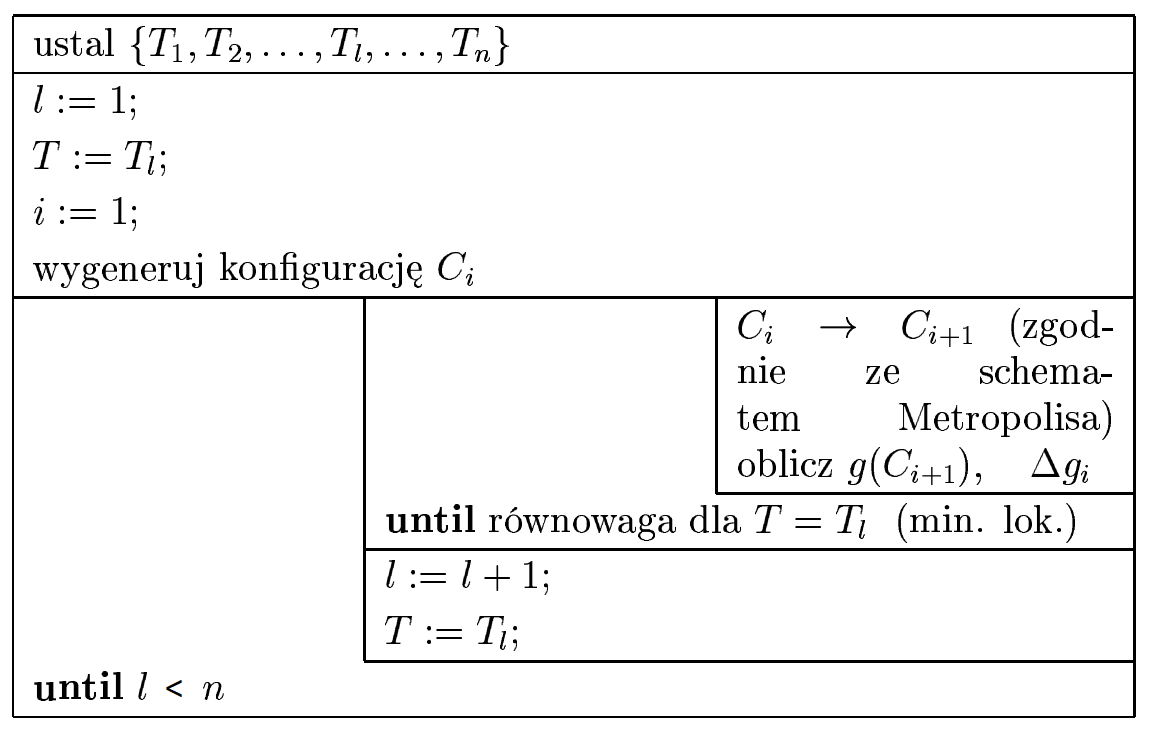
\includegraphics[width=0.8\textwidth]{img/18/sa_algorithm}
		\end{figure}
		$\{T_l\}$ - temperature schedule: $T_l > T_{l+1}$\\
		np. $T_{l+1} = 0.9 \cdot T_l$
	\end{frame}

	\begin{frame}{Fundamentalny fakt z mechaniki statystycznej}
		Załóżmy, że układ znajduje się w równowadze termicznej (w temperaturze $T$)\\
	Prawdopodobieństwo, że układ znajduje się w mikrostanie  stanie $\alpha$ jest proporcjonalne do {\bf czynnika Boltzmanna}  $$e^{\frac{-E_\alpha}{k_B T}}$$\\
		gdzie: $E_\alpha$ - energia stanu
	
		
		
	\end{frame}

%%%%%%%%%%%%%%%%

	\begin{frame}{Schemat Metropolisa}
		\textbf{Podstawa metody Monte Carlo symulacji molekularnej}
		\begin{figure}
			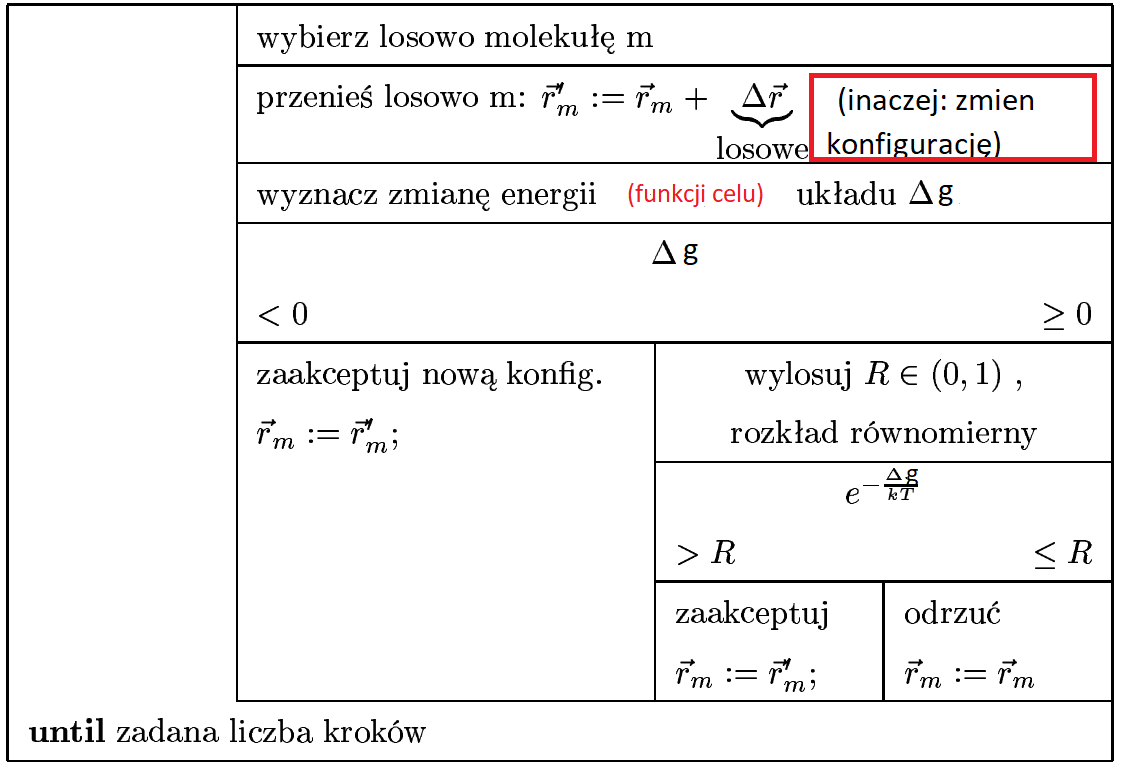
\includegraphics[width=0.67\textwidth]{img/18/metropolis1}
		\end{figure}
		\begin{thebibliography}{9}
			\setbeamertemplate{bibliography item}[article]
			\bibitem{metropolis}{Nicolas Metropolis, Arianna W. Rosenbluth, Marshal M. Rosenbluth, Augusta H. Teller, Edward Teller \newblock J. Chem. Phys. 21 (1953) 1087}
		\end{thebibliography}
	\end{frame}
		\begin{frame}{Sprawdzanie, czy układ jest w równowadze}
		\begin{block}{Sposób A}
			utrzymywać $T_l$ przez $\begin{cases}
			100 \cdot N \text{ prób} \\
			10 \cdot N \text{ prób udanych} (\Delta g < 0)
			\end{cases}$
		\end{block}
		
		\begin{block}{Sposób B}
		$n$ - ustalona liczba prób ($\sim$ epoka)
		\begin{enumerate}
			\item wykonać $n$ prób ($C_i \rightarrow C_{i+1}$)
			\item zachować g(C$_n$)
			\item porównać $g_i(C_n)$ dla kilku ostatnich zestawów po $n$ próbach \\
			brak istotnej zmiany $g(C_n) \rightarrow$ nowe $T$.
		\end{enumerate}
		\end{block}
\end{frame}
\begin{frame}{Wartość początkowa T}
\begin{itemize}
    \item wystarczająco wysoka by zapewnić akceptację niemal wszyskich przejść
    \item wartość początkowa parametru T zależy od postawionego problemu
    \item np. przyjąć jakiś wstępną wartość prawdopodobieństwa $P\approx 1$  i dla losowej próby wyliczyć średnią różnicę pomiędzy
    $\Delta g=g(C_i)-g(C_j)$
    \item wybrać $T_0=-\frac{\Delta g}{ln(P)}$
\end{itemize}
		   
			
		
		
\end{frame}
		\begin{frame}{Charakterystyka schematu Metropolisa}
		\begin{itemize}
			\item $T \nearrow$ - łatwiej akceptowalne kroki z $g(C_i) \nearrow (E)$ \\ $ \Rightarrow$ możliwość opuszczenia stanu metastabilnego (lokalnego minimum).
			\item zmiany $g(C_i) \searrow$ są akceptowane zawsze
		\end{itemize}
		
		Po wielu krokach system $\rightarrow$ stan równowagi termodynamicznej z parametrami oscylującymi wokół wartości średnich zgodnie z rozkładem Boltzmanna 
		

	\end{frame}

%%%%%%%%%%%%%%%%
%	\begin{frame}{Interaktywna demonstracja działania Simulated Annealing}
%		Źródła w C i C++:
%		\begin{itemize}
	%		\item 	%\url{https://www.taygeta.com/annealing/simanneal.html}
%		\end{itemize}
		
		
		%Programy w C:
		%Postscript:
		% martwe linki
%	\end{frame}
	%%%%%%%%%%%%%%%%%%%%%%%
	%\section{Schemat Metropolisa}

%%%%%%%%%%%%%%%%


%%%%%%%%%%%%%%%%

%	\begin{frame}{Schemat Metropolisa}
%		$$
%			\Delta \vec{r} = \delta(\vec{i} \cdot a_x + \vec{j} \cdot a_y  + \vec{k} \cdot a_z)
%		$$		
%		
%		$$
%		\delta \text{ - wybrane z góry} \approx 10^{-11}m
%		$$		
		
%		$$
%		a_i \in (-1, 1), Unif
%		$$
		
	%	\begin{figure}
			%\includegraphics[width=0.5\textwidth]{img/18/metropolis2}
	%	\end{figure}
	%	$a_i$, R - liczby pseudolosowe
		
	%	$\Delta\phi$ - zmiana energii potencjalnej układu w wyniku przesunięcia molekuły m
		
		%Dead link
		%Aplet metropolis/metropolis.html 
%	\end{frame}

%%%%%%%%%%%%%%%%
	
	\begin{frame}{Charakterystyka schematu Metropolisa}
		\begin{itemize}
			\item $T \nearrow$ - łatwiej akceptowalne kroki z $g(C_i) \nearrow (E)$ \\ $ \Rightarrow$ możliwość opuszczenia stanu metastabilnego (lokalnego minimum).
			\item zmiany $g(C_i) \searrow$ są akceptowane zawsze
		\end{itemize}
		
		Po wielu krokach system $\rightarrow$ stan równowagi termodynamicznej z parametrami oscylującymi wokół wartości średnich zgodnie z rozkładem Boltzmanna 
		

	\end{frame}

\subsection{Łańcuch Markowa}
%%%%%%%%%%%%%%%%
	
	\begin{frame}{Schemat Metropolisa $\rightarrow$ łańcuch Markowa}
		\begin{figure}
				\includegraphics[width=0.5\textwidth]{img/18/markow}
		\end{figure}
		\begin{block}{Zasada równowagi szczegółówej\\ 
		(detailed balance, microscopic reversibility)}
			$$
			p_2 \cdot 1 = p_1 \cdot e^{- \dfrac{E_2 - E_1}{kT}}
			$$
		\end{block}
	\end{frame}

%%%%%%%%%%%%%%%%
	\begin{frame}{Łańcuch Markowa}
		$$
	 	\frac{p1}{p2} = \dfrac{e^{-\frac{E_1}{kT}}}{e^{-\frac{E_2}{kT}}} \rightarrow p_i \sim \underbrace{e^{-\frac{E_i}{kT}}}_{\text{czynnik prawdop. Boltzmanna}}
		$$		
		
		$$
		P(c_i) \sim e^{-\frac{E_i}{kT}}
		$$
		
		$\Rightarrow$ importance sampling: konfiguracje generowane nie losowo - ale z zadanym rozkładem (50-70 \% akceptowanych)
		%Dead link
		%	Notatka nt. niejednorodnych łańcuchów Markowa w SA, dużo bibliografii
		
		% whaaaat
		% http://www.pz.zgora.pl/discuss/al15_2/a6.htm
		
	\end{frame}
	
\section{Uwagi praktyczne}
%%%%%%%%%%%%%%%%
\begin{frame}{Symulacja molekularna - uwagi praktyczne}
		\textbf{Duże $\Delta\vec{r}$:}
		\begin{itemize}
			\item niski poziom akceptacji
			\item szybsze próbkowanie przestrzeni konfiguracyjnej
		\end{itemize}
		
		\textbf{Dla potencjałów parowych, krótkozasięgowych:}
		\begin{itemize}
			\item przesuwamy tylko 1 cząstkę
			\item dla określenia $\Delta\phi$ - tylko najbliżsi sąsiedzi
		\end{itemize}
		
		\textbf{W przypadku cieczy:}
		\begin{itemize}
			\item każda cząsteczka $\approx 10^3$ przemieszczeń
			\item w modelu $\approx 10^3$ cząsteczek
		\end{itemize}	
		
		\textbf{Force-biased displacement:}
		\begin{itemize}
			\item wszystkie cząsteczki przesuwane równocześnie przeciwnie do gradientu potencjału
		\end{itemize}
		
	\end{frame}

	%%%%%%%%%%%%%%%%%%%%%%%
	%\input{18_simulated_annealing/18_7_sa_rozklad}
	%%%%%%%%%%%%%%%%%%%%%%%
	\input{18_simulated_annealing/18_8_zastosowania}
	%%%%%%%%%%%%%%%%%%%%%%%
	\input{18_simulated_annealing/18_9_odmiany}
	%%%%%%%%%%%%%%%%%%%%%%%
	\input{18_simulated_annealing/18_10_literatura}
	%\section{Wyżarzacz kwantowy}
\begin{frame}
\frametitle{Wyżarzacz kwantowy D-Wave
 }


\begin{itemize}
\item metaheurystyka do znajdowania globalnego minimum 
\item tunelowanie kwantowe (wyjście z minimum lokalnego)
\end{itemize}

\begin{figure}
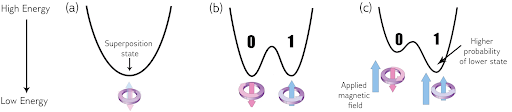
\includegraphics[scale=0.4]{img/18/gorki.png}
\caption{Zmiany energii podczas kwantowego wyżarzania\\source: \url{https://docs.dwavesys.com/docs/latest/c_gs_2.html}}
\end{figure}

\end{frame}
\begin{frame}{Notacja Diraca, iloczyn tensorowy}
  $$\ket{0}=\begin{bmatrix}1\\0
        \end{bmatrix}
        \ket{1}=\begin{bmatrix}0\\1
        \end{bmatrix}$$ 
       $$\ket{00}=\begin{bmatrix}1\\0\\0\\0
       \end{bmatrix}
        \ket{01}=\begin{bmatrix}0\\1\\0\\0
        \end{bmatrix}
        \ket{10}=\begin{bmatrix}0\\0\\1\\0
        \end{bmatrix}
       \ket{11}=\begin{bmatrix}0\\0\\0\\1
       \end{bmatrix}$$ 
        $$\ket{01}=\ket{0}\otimes\ket{1}=
        \begin{bmatrix}1\\0
        \end{bmatrix}\otimes
\begin{bmatrix}0\\1
        \end{bmatrix}=
       \begin{bmatrix}1\cdot0\\1\cdot1\\0\cdot0\\0\cdot1
        \end{bmatrix}=\begin{bmatrix}0\\1\\0\\0
        \end{bmatrix}$$
        
\end{frame}
\begin{frame}{Kwantowy Hamiltonian dla MaxCut}
Funkcja kosztu:
    \begin{itemize}
        \item[] $g(x_1, x_2)=x_1+x_2-2x_1 x_2$, $x_1,x_2 \in\{0,1\}$
        \item[] $x\rightarrow \frac{1}{2}(1-z)$  
        \item[] $g(z_1,z_2)=\frac{1}{2}(1-z_1z_2)$ $z_1,z_2 \in\{-1,1\}$
        \item[]
        $\sigma_z=\begin{pmatrix}  
    1 &0\\
    0 & -1\\
    \end{pmatrix}$
        \item[] $\sigma_z\ket{0}=\ket{0}, \lambda=1$
       \item[] $\sigma_z\ket{1}=-\ket{1}, \lambda=-1$
       \item[] aby zbudować Hamiltonian: $z\rightarrow \sigma_z$
        \item[] $H_{i,j}=\frac{1}{2}(I-{\sigma_z}^i\otimes {\sigma_z}^j)=\begin{pmatrix}  
    0 &0&0&0\\
     0 &1&0&0\\
      0 &0&1&0\\
       0 &0&0&0
    \end{pmatrix} \begin{matrix}
    \ket{00}\\
     \ket{01}\\
      \ket{10}\\
       \ket{11}\\
    \end{matrix}$
        \item[]Wartości włąsne
        \begin{itemize}
            \item $0$ dla $\ket{00}$ i $\ket{11}$ ; $g(00)=0$ $g(11)=0$
             \item $1$ dla $\ket{01}$ i $\ket{10}$ ; $g(01)=1$ $g(10)=1$
        \end{itemize}
    \end{itemize}
    \\
    \small{source: https://grove-docs.readthedocs.io/en/latest/qaoa.html}
\end{frame}
\begin{frame}
\frametitle{Quantum Annealing}
\small
%\begin{columns}[t] % The "c" option specifies centered vertical alignment while the "t" option is used for top vertical alignment
%\column{.5\textwidth} % Left column and width
\begin{itemize}
\item 
startuje w stanie o najniższej energii początkowego H
\item powoli zmienia początkowy H w H dla naszego problemu
\item zmiana dokonuje sie poprzez wprowadzenie  tzw  couplers (J) oraz biases (h) 
\item w idealnej sytuacji system pozostaje w stanie o minimalnej energii przez cały ten proces 
 
 \item działanie kończy się, gdy system znajduje się w stanie o minimalnej energii dla naszego problemu
\item wynik zwracany jest jako klasyczna wartość
\end{itemize}


$$\underbrace{- \frac{A({s})}{2} \left(\sum_i {\sigma_{x}^{(i)}}\right)}_\text{Initial Hamiltonian} + \underbrace{\frac{B({s})}{2} \left(\sum_{i} h_i {\sigma_{z}^{(i)}} + \sum_{i>j} J_{i,j} {\sigma_{z}^{(i)}} {\sigma_{z}^{(j)}}\right)}_\text{Final Hamiltonian}$$

\end{frame}
\begin{frame}{Co należy zrobić?}
 \begin{itemize}
     \item sformułuj problem jako QUBO
\item dopasuj QUBO do architektury komputera
\item otrzymaj rezultaty 
\item dokonaj odwrotnego dopasowania wyników do początkowego QUBO
 \end{itemize}   
\end{frame}

\begin{frame}{QUBO i Hamiltonian}
\begin{block}{QUBO - quadratic and uncontraint cost function $f(x)=x^TQx$}
$f(x)=x^TCx+P\underbrace{(Ax-b)^T(Ax-b)}_{\substack{\text{instead of solving } Ax=b \\ \text{we minimize inner product of }
Ax-b
}}$ 
\end{block}
   $x_i \rightarrow \frac{I-{\sigma_z}^i}{2}$ \arrowupdown  ${\sigma_z}^i= I\otimes I\dots\otimes\underbrace{\sigma_z}_{\text{i- th position}}\dots\otimes I$\\
  
\begin{block}{Hamiltonian}
$H=\sum_{i}c_i\frac{I-{\sigma_z}^i}{2}+P\sum_j (\sum_ia_{j,i}(I-\frac{{\sigma_z}^i}{2})-b_iI)^2$
\end{block} 
Obydwie formy mogą być wejsciem do wyżarzacza kwantowego
\end{frame}

\begin{frame}{Minor Embedding}
 \begin{columns}[t] % The "c" option specifies centered vertical alignment while the "t" option is used for top vertical alignment
\column{.7\textwidth} 
\begin{itemize}
    \item Architektura kwantowego wyżarzacza nie jest grafem pełnym
    
\item konieczna jest transformacja grafu naszego problemu do tej architektury 
\item  zwykle konieczne jest reprezentowanie jednej zmiennej problemu przez wiele qbitów (łańcuchy)

\end{itemize}
\column{.3\textwidth} 
    \begin{figure}[H]
    \centering
    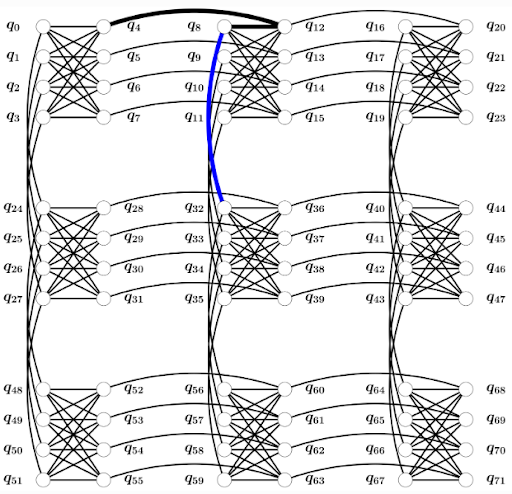
\includegraphics[width=\linewidth]{img/18/chimera.png}
\end{figure}

\end{columns}
 \begin{figure}[H]
    \centering
    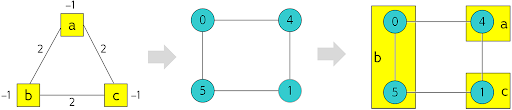
\includegraphics[width=0.9\linewidth]{img/18/simple_embed.png}
\end{figure} 
\tiny Source: https://docs.dwavesys.com/docs/latest/c\_gs\_7.html

\end{frame}
\begin{frame}{Embedowanie pełnego grafu}
\begin{itemize}
    \item przykład jak osadzić graf $K_9$ w grafie Chimera $2\times2$
\item trzy qbity na jedną zmienną  (poza 8)
\item ta metoda działa dla grafów do 9 wierzchołków

\end{itemize}    
\begin{figure}[H]
    \centering
    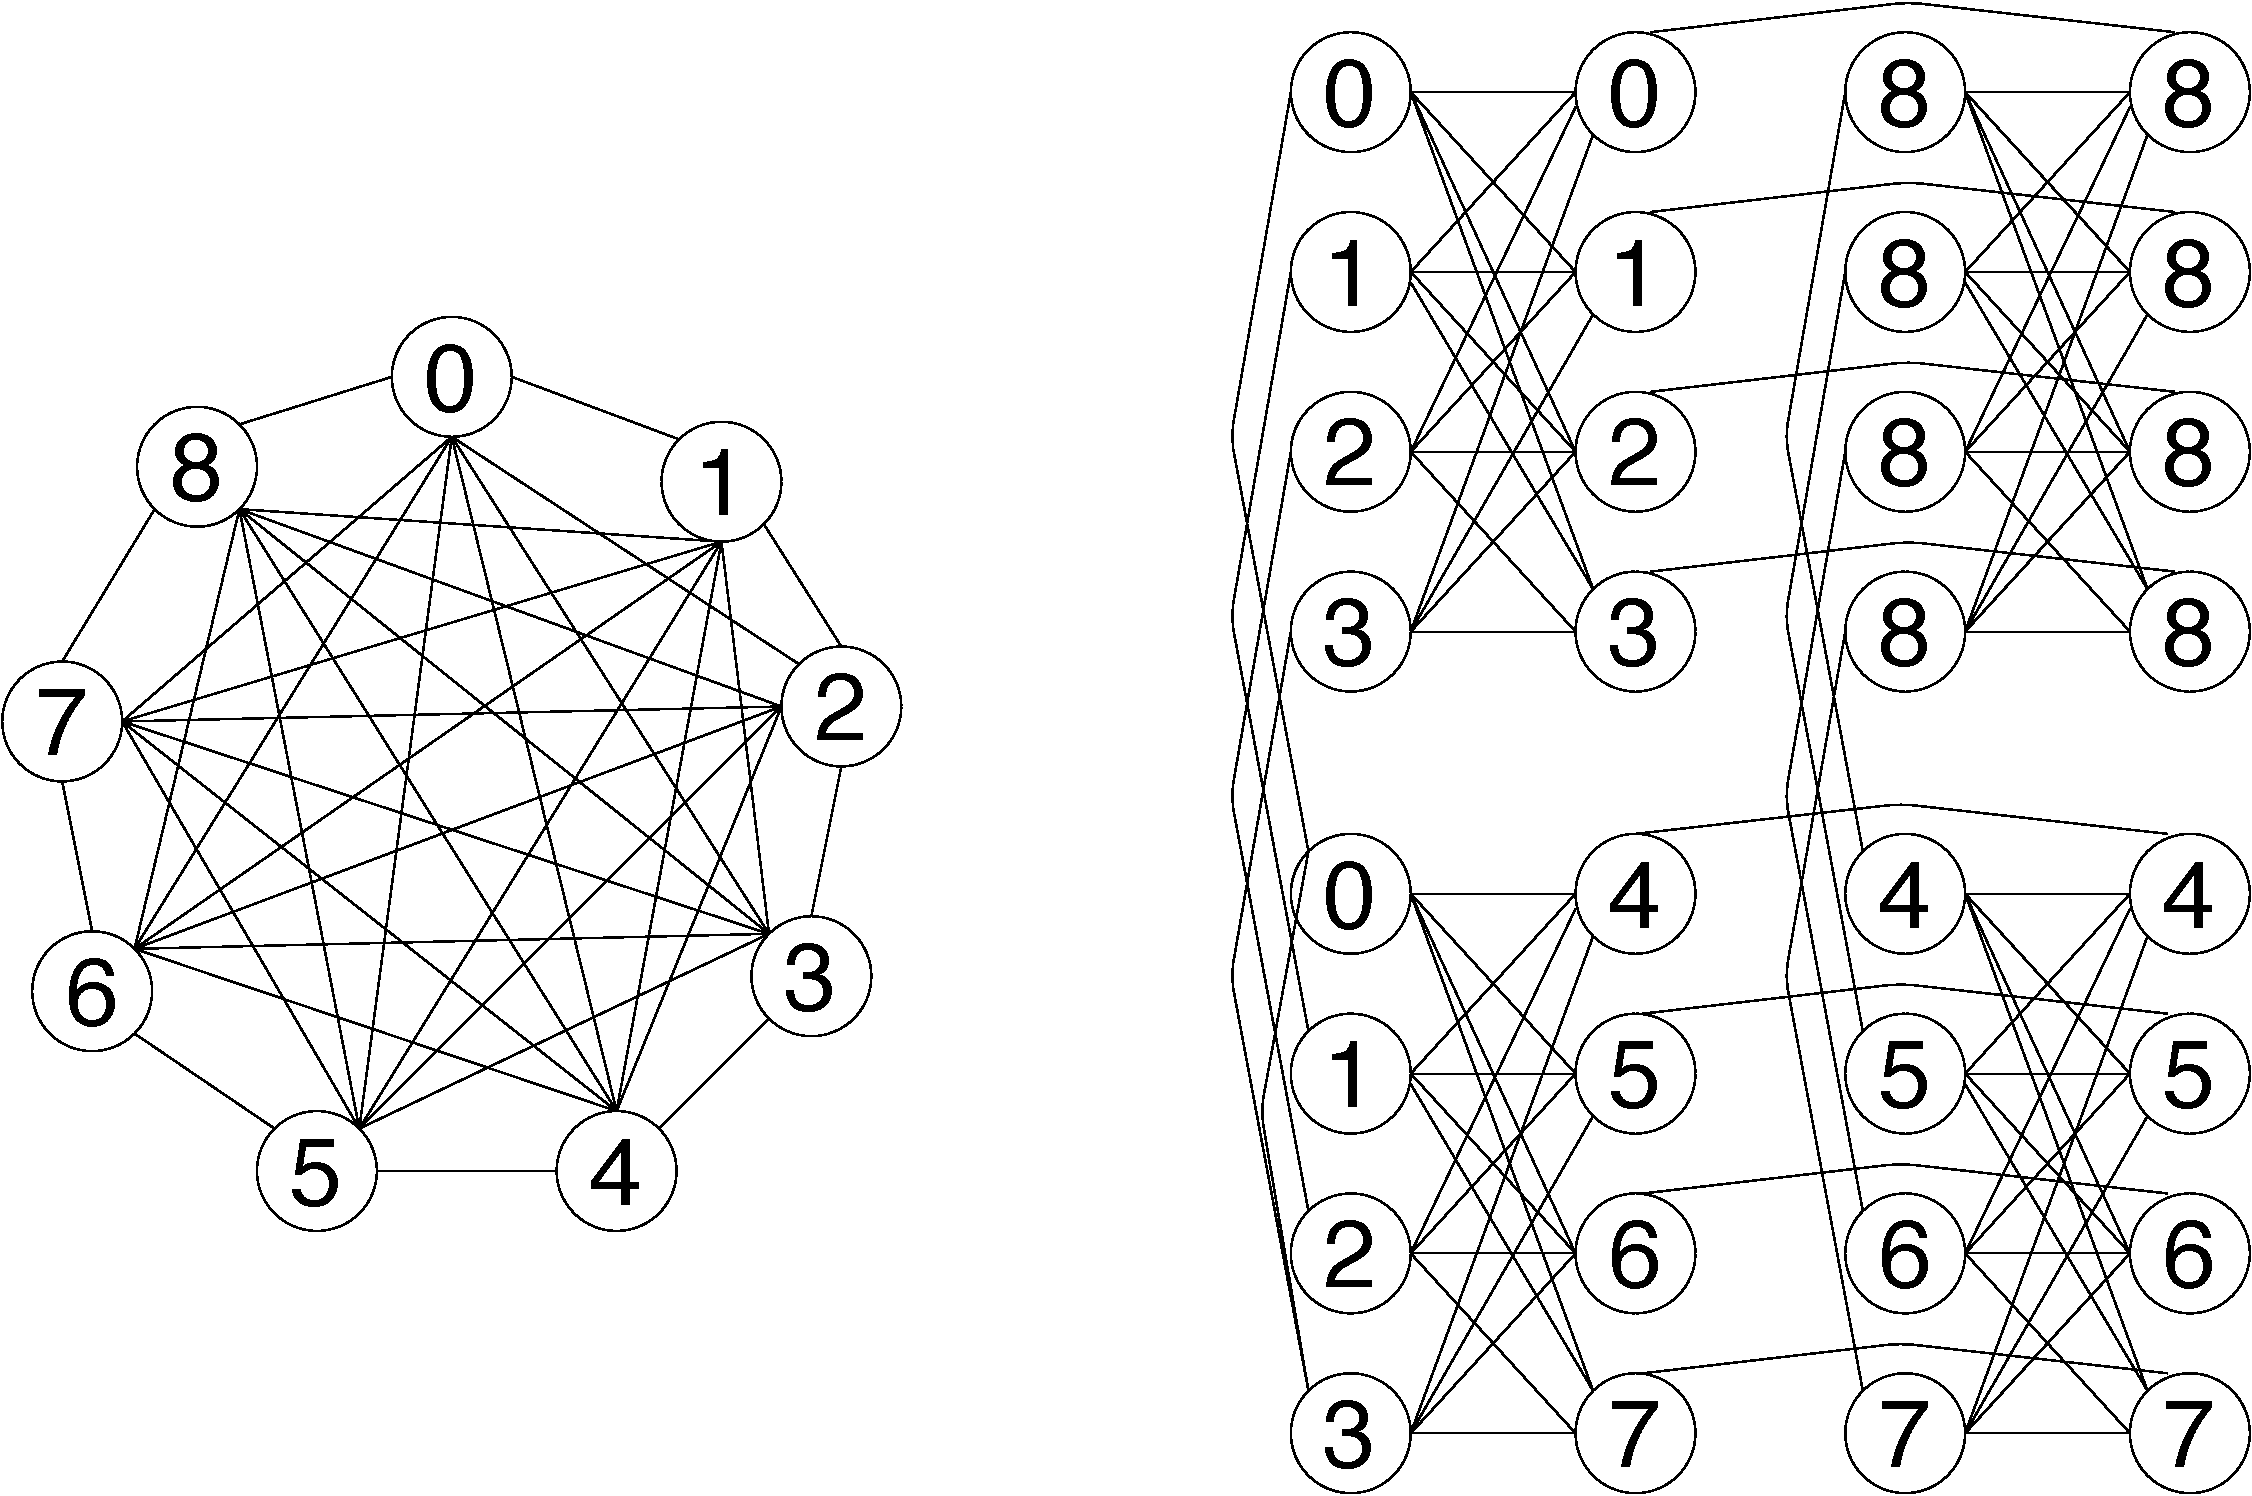
\includegraphics[width=0.5\linewidth]{img/18/complete_chimera_k9_v2.pdf}
\end{figure} 
\end{frame}


\end{document}
